\documentclass[letterpaper,14pt]{extarticle}
\usepackage[margin=0.65in,top=0.73in,bottom=0.69in,headheight=17pt,headsep=17pt]{geometry}
\usepackage[T1]{fontenc}
\usepackage[scaled=0.94]{helvet}
\renewcommand{\familydefault}{\sfdefault}
\usepackage{tikz}
\usetikzlibrary{arrows.meta}
\usepackage{fancyhdr}
\usepackage{xcolor}
\usepackage{microtype}
\definecolor{braceblue}{RGB}{20,73,112}
\definecolor{softgray}{RGB}{130,130,130}
\pagestyle{fancy}
\fancyhf{}
\renewcommand{\headrulewidth}{0pt}
\renewcommand{\footrulewidth}{0pt}
\fancyfoot[L]{\fontsize{9}{11}\selectfont Bellingham Math Circle / Week 52 / F52-S-v2}
\fancyfoot[R]{\fontsize{9}{11}\selectfont\thepage}
\setlength{\parindent}{0pt}
\setlength{\parskip}{8pt}
\newcommand{\band}[1]{\fancyhead[L]{\fontsize{11.5}{14}\selectfont Week 52 / Hinged frames and braces / #1}}
\newcommand{\problem}[2]{\par\textbf{Problem #1:} #2\par}
\newcommand{\spacebox}[2]{\begin{tikzpicture}\draw[softgray,densely dotted,line width=0.6pt] (0,0) rectangle (#1,#2);\end{tikzpicture}}
% Grid row numbers run from the top. Braces are r/c pairs.
% Every grid uses the same x and y unit: all initial cells are squares.
\newcommand{\gridpic}[5]{%
  \begin{tikzpicture}[x=#3mm,y=#3mm,baseline=(current bounding box.center)]
    \foreach \x in {0,...,#2}{\draw[line width=0.9pt] (\x,0)--(\x,#1);}
    \foreach \y in {0,...,#1}{\draw[line width=0.9pt] (0,\y)--(#2,\y);}
    \foreach \r/\c in {#4}{\draw[braceblue,line width=2pt] ({\c-1},{#1-\r})--(\c,{#1-\r+1});}
    \foreach \x in {0,...,#2}{\foreach \y in {0,...,#1}{\filldraw[fill=white,line width=0.65pt] (\x,\y) circle (2.2pt);}}
    \ifnum#5=1
      \foreach \r in {1,...,#1}{\node[anchor=east,font=\fontsize{11}{13}\selectfont] at (-0.13,{#1-\r+0.5}) {R\r};}
      \foreach \c in {1,...,#2}{\node[anchor=south,font=\fontsize{11}{13}\selectfont] at ({\c-0.5},{#1+0.11}) {C\c};}
    \fi
  \end{tikzpicture}%
}
% Link graph has strip vertices rather than physical joints.
\newcommand{\linkpic}[4]{%
  \begin{tikzpicture}[x=1cm,y=1cm,baseline=(current bounding box.center)]
    \pgfmathsetmacro{\maxnum}{max(#1,#2)}
    \foreach \r in {1,...,#1}{\coordinate (R\r) at (0,{(\maxnum-\r)*0.85});}
    \foreach \c in {1,...,#2}{\coordinate (C\c) at (#3,{(\maxnum-\c)*0.85});}
    \foreach \r/\c in {#4}{\draw[braceblue,line width=1.5pt] (R\r)--(C\c);}
    \foreach \r in {1,...,#1}{\filldraw[fill=white,line width=0.8pt] (R\r) circle (2.7pt);\node[anchor=east,font=\fontsize{11}{13}\selectfont] at (-0.15,{(\maxnum-\r)*0.85}) {R\r};}
    \foreach \c in {1,...,#2}{\filldraw[fill=white,line width=0.8pt] (C\c) circle (2.7pt);\node[anchor=west,font=\fontsize{11}{13}\selectfont] at ({#3+0.15},{(\maxnum-\c)*0.85}) {C\c};}
  \end{tikzpicture}%
}
\newcommand{\recordgrid}[2]{\gridpic{#1}{#2}{21}{}{0}}
\newcommand{\casegrid}[3]{\begin{minipage}[t]{0.46\linewidth}\centering #1\par\vspace{4pt}\gridpic{2}{2}{23}{#2}{0}\par\vspace{12pt}\spacebox{5.7}{#3}\end{minipage}}
\newcommand{\lines}[1]{\foreach \i in {1,...,#1}{\noindent\rule{\linewidth}{0.3pt}\par\vspace{15pt}}}
\begin{document}
\band{Grades K--1}
\fontsize{16}{21}\selectfont
Keep the frames flat. Bars stay straight and keep their length; joints may turn. Sliding or turning the whole frame does not change its shape.

Drawings are recording maps.

\problem{1}{Can you change the shape of the triangle and the square? Draw the shapes you can make.}
\vspace{12pt}
\begin{minipage}[t]{0.46\linewidth}\centering
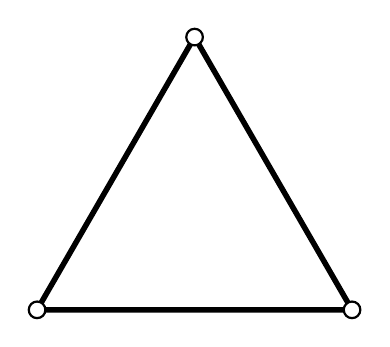
\begin{tikzpicture}[x=1cm,y=1cm]
\draw[line width=2pt] (0,0)--(4,0)--(2,3.4641)--cycle;
\foreach \p in {(0,0),(4,0),(2,3.4641)}{\filldraw[fill=white,line width=0.8pt] \p circle (3pt);}
\end{tikzpicture}
\par\vspace{18pt}\spacebox{7.2}{5.6}
\end{minipage}\hfill
\begin{minipage}[t]{0.46\linewidth}\centering
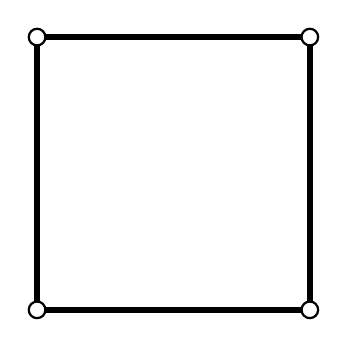
\begin{tikzpicture}[x=1cm,y=1cm]
\draw[line width=2pt] (0,0) rectangle (3.4641,3.4641);
\foreach \p in {(0,0),(3.4641,0),(3.4641,3.4641),(0,3.4641)}{\filldraw[fill=white,line width=0.8pt] \p circle (3pt);}
\end{tikzpicture}
\par\vspace{18pt}\spacebox{7.2}{5.6}
\end{minipage}

\newpage
\band{Grades K--1}
\problem{2}{Make the square hold its shape with the fewest diagonal bars. Draw where you put the bars.}
A diagonal bar joins opposite corner pins. It is called a brace.
\vspace{20pt}
\begin{center}
\gridpic{1}{1}{50}{}{0}\hspace{30mm}\gridpic{1}{1}{50}{}{0}
\end{center}
\vspace{12pt}
\problem{3}{Remove the diagonal and make shapes with the four side bars. Which shapes can you fit that same diagonal into?}
\vspace{13pt}
\begin{center}\spacebox{15.8}{7}\end{center}

\newpage
\band{Grades 2--3}
\fontsize{14}{19}\selectfont
In a grid, use at most one diagonal brace in each cell.
\problem{4}{Build these designs on your 2-by-2 frame. Circle each design that holds its shape. For each frame that can change shape, draw a changed shape.}
\vspace{11pt}
\casegrid{A}{1/1}{3.7}\hfill\casegrid{B}{1/1,2/2}{3.7}
\par\vspace{17pt}
\casegrid{C}{1/1,1/2,2/1}{3.7}\hfill\casegrid{D}{1/1,1/2,2/1,2/2}{3.7}

\newpage
\band{Grades 2--3}
\problem{5}{Find the fewest braces that make your 2-by-2 frame hold its shape. Find several designs using that many braces.}
\vspace{5pt}
Fewest braces: \rule{22mm}{0.4pt}
\vspace{20pt}
\begin{center}
\recordgrid{2}{2}\hspace{25mm}\recordgrid{2}{2}
\par\vspace{25mm}
\recordgrid{2}{2}\hspace{25mm}\recordgrid{2}{2}
\end{center}

\newpage
\band{Grades 3--5}
\problem{6}{Find the fewest braces that make your 2-by-3 frame hold its shape. Find several designs using that many braces.}
\vspace{5pt}
Fewest braces: \rule{22mm}{0.4pt}
\vspace{18pt}
\begin{center}
\recordgrid{2}{3}\hspace{14mm}\recordgrid{2}{3}
\par\vspace{24mm}
\recordgrid{2}{3}\hspace{14mm}\recordgrid{2}{3}
\end{center}

\newpage
\band{Grades 3--5}
\fontsize{13.5}{18}\selectfont
A brace becomes a link between its row dot and its column dot. Keep all the dots. Links may cross; a crossing is not a dot.
\vspace{5pt}
\begin{center}
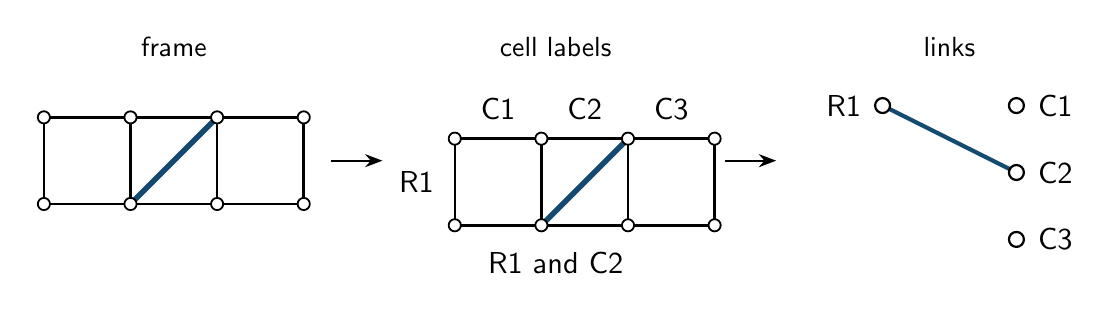
\begin{tikzpicture}[x=1cm,y=1cm]
\node at (2.15,1.45) {frame};
\node at (7.0,1.45) {cell labels};
\node at (12.0,1.45) {links};
\node at (2.15,0) {\gridpic{1}{3}{11}{1/2}{0}};
\node at (7.0,0) {\gridpic{1}{3}{11}{1/2}{1}};
\node at (12.0,-0.15) {\linkpic{1}{3}{1.7}{1/2}};
\draw[-{Stealth[length=2.2mm]},line width=0.8pt] (4.15,0)--(4.8,0);
\draw[-{Stealth[length=2.2mm]},line width=0.8pt] (9.15,0)--(9.8,0);
\node[font=\fontsize{11}{13}\selectfont] at (7.0,-1.3) {R1 and C2};
\end{tikzpicture}
\end{center}
\problem{7}{Make A and B on your 2-by-3 frame. Draw their links. Circle each design that holds its shape.}
\vspace{9pt}
\begin{minipage}{0.46\linewidth}\centering A\par\vspace{4pt}
\gridpic{2}{3}{18}{1/1,1/2,2/1,2/2}{1}
\par\vspace{15mm}\linkpic{2}{3}{3}{}
\end{minipage}\hfill
\begin{minipage}{0.46\linewidth}\centering B\par\vspace{4pt}
\gridpic{2}{3}{18}{1/1,1/2,1/3,2/1}{1}
\par\vspace{15mm}\linkpic{2}{3}{3}{}
\end{minipage}

\newpage
\band{Grades 3--5}
\fontsize{14}{19}\selectfont
\problem{8}{Does putting a brace in every row and every column always make a frame hold its shape? Draw A and B's links and decide.}
\vspace{14pt}
\begin{minipage}{0.46\linewidth}\centering A\par\vspace{4pt}
\gridpic{3}{3}{20}{1/1,1/2,2/1,2/2,3/3}{1}
\par\vspace{12mm}\linkpic{3}{3}{3.1}{}
\end{minipage}\hfill
\begin{minipage}{0.46\linewidth}\centering B\par\vspace{4pt}
\gridpic{3}{3}{20}{1/1,1/2,1/3,2/1,3/1}{1}
\par\vspace{12mm}\linkpic{3}{3}{3.1}{}
\end{minipage}
\par\vspace{30pt}
\lines{3}

\newpage
\band{Grades 3--5}
\problem{9}{Find every single brace you can remove from this design while the frame still holds its shape. Replace it before testing another. Mark those braces on both pictures.}
\vspace{12pt}
\begin{center}
\gridpic{2}{3}{26}{1/1,1/2,1/3,2/1,2/2}{1}
\hspace{20mm}\linkpic{2}{3}{3.6}{1/1,1/2,1/3,2/1,2/2}
\end{center}
\vspace{14pt}
\problem{10}{Starting with all six cells braced, find pairs you can remove while the frame still holds its shape, and pairs that let it change shape. Cross out the removed braces and circle each design that holds its shape.}
\vspace{8pt}
\begin{center}
\gridpic{2}{3}{17}{1/1,1/2,1/3,2/1,2/2,2/3}{1}\hspace{25mm}\gridpic{2}{3}{17}{1/1,1/2,1/3,2/1,2/2,2/3}{1}
\par\vspace{10mm}
\gridpic{2}{3}{17}{1/1,1/2,1/3,2/1,2/2,2/3}{1}\hspace{25mm}\gridpic{2}{3}{17}{1/1,1/2,1/3,2/1,2/2,2/3}{1}
\end{center}

\newpage
\band{Grades 3--5}
\problem{11}{Can one new brace make each frame hold its shape? Mark every place that works.}
\vspace{14pt}
\begin{minipage}{0.46\linewidth}\centering A\par\vspace{4pt}
\gridpic{3}{3}{20}{1/1,1/2,2/1,2/2}{1}
\par\vspace{12mm}\linkpic{3}{3}{3.1}{}
\end{minipage}\hfill
\begin{minipage}{0.46\linewidth}\centering B\par\vspace{4pt}
\gridpic{3}{3}{20}{1/1,1/2,2/2,3/3}{1}
\par\vspace{12mm}\linkpic{3}{3}{3.1}{}
\end{minipage}
\par\vspace{34pt}
\lines{3}

\newpage
\band{Grades 4--5}
\problem{12}{Find the fewest braces that make a 4-by-5 grid hold its shape. Draw a design using that many, and explain why fewer cannot work.}
\vspace{5pt}
Fewest braces: \rule{22mm}{0.4pt}
\vspace{16pt}
\begin{center}\gridpic{4}{5}{21}{}{1}\end{center}
\vspace{18pt}
\lines{4}

\newpage
\band{Grades 4--5}
\problem{13}{A 3-by-3 grid has six braces, with a brace in every row and column. Must it hold its shape? Explain.}
\vspace{7pt}
\begin{center}\gridpic{3}{3}{19}{}{1}\hspace{23mm}\gridpic{3}{3}{19}{}{1}\end{center}
\vspace{12pt}
\lines{2}
\newpage
\band{Grades 4--5}
\problem{14}{A 4-by-4 grid has nine braces, with a brace in every row and column. Must it hold its shape? Explain.}
\vspace{16pt}
\begin{center}\gridpic{4}{4}{23}{}{1}\end{center}
\vspace{20pt}
\lines{4}
\end{document}
